\documentclass[11pt]{article}
\usepackage[margin=21mm]{geometry}
\usepackage{amsmath,booktabs,graphicx}
\begin{document}
\title{Event-total ion and photon fluctuations: 100 bb0nu events}
\author{NAUSICAA generated analysis report}
\date{}\maketitle
\section*{Question and sample}
The analysis includes 100 bb0nu events from the 1 mm Geant4 hit table. Their mean expected primary-pair count is 112,229.689; its across-event standard deviation is 0.0009. Its mean energy is 2.457830 MeV, effectively fixed across events for this comparison.
\section*{Method and conditions}
At each hit $\mu_i=10^6E_i/W$, with $W=21.90$ eV and $F=0.150$. The minimum integer variance gives $V_{\rm pair}=\sum_i\max[F\mu_i,\{\mu_i\}(1-\{\mu_i\})]$. The ion branch collects every primary ion, so its event total is the pair draw. The photon branches use $J=0.010$, optical acceptance $A=0.19098$, and EL yields $Y_{\rm Xe}=2,332.4$ and $Y_{\rm XeHe}=2,293.5$ photons per surviving electron. The yield and acceptance are fixed model inputs; photons touching the EL-hole wall are absorbed.
\[p=\exp[-L_e/(v_e\tau_e)],\qquad \widehat E_{\gamma}=\frac{W}{10^6}\,\frac{N_{\gamma,\mathrm{incident}}}{pYA}\quad\mathrm{MeV}.\]
The photon energy estimator is corrected separately for each event's known drift length. Only the corrected estimator minus that event's deposited energy enters the measured width. The correction removes the drift-dependent mean. For a fixed pair count $N$, binomial attachment still gives $\operatorname{Var}(N_{\rm survive}/p\mid N)=N(1-p)/p$. On the primary-pair scale, the predicted conditional variance is
\[V_{\gamma,\mathrm{eq}}=V_{\rm pair}+\mu\frac{1-p}{p}+\frac{J\mu}{pY}+\frac{\mu(1-A)}{pYA}.\]
These terms represent pair creation, attachment, EL emission and optical collection. The two gas branches share the primary pair and attachment draws. No PDE or electronics response is applied.
Electron survival spans 0.9111--0.9987 across sampled drift lengths.
\section*{Results}
\begin{center}\begin{tabular}{lrrrr}\toprule
Energy estimator & SD obs. (keV) & SD model (keV) & SD obs. (\%) & SD model (\%)\\\midrule
Ions & 2.70 & 2.84 & 0.1098 & 0.1156\\
Pure-Xe photons, corrected & 3.31 & 3.32 & 0.1346 & 0.1352\\
Xe--He photons, corrected & 3.27 & 3.32 & 0.1332 & 0.1352\\
\bottomrule\end{tabular}\end{center}
For 100 independent events, the relative sampling uncertainty of an SD is approximately 7\%, so the observed and predicted widths agree at this sample size.
The corrected energy-residual correlation with drift length is 0.065 (pure Xe) and 0.046 (Xe--He).
\begin{center}\begin{tabular}{lrr}\toprule
Mean variance term (pair count$^2$) & Pure Xe & Xe--He\\\midrule
Fano/integer pairs & 16,834.8 & 16,834.8\\
Attachment & 5,961.4 & 5,961.4\\
EL emission & 0.5 & 0.5\\
Optical collection & 214.7 & 218.3\\
\bottomrule\end{tabular}\end{center}
\begin{center}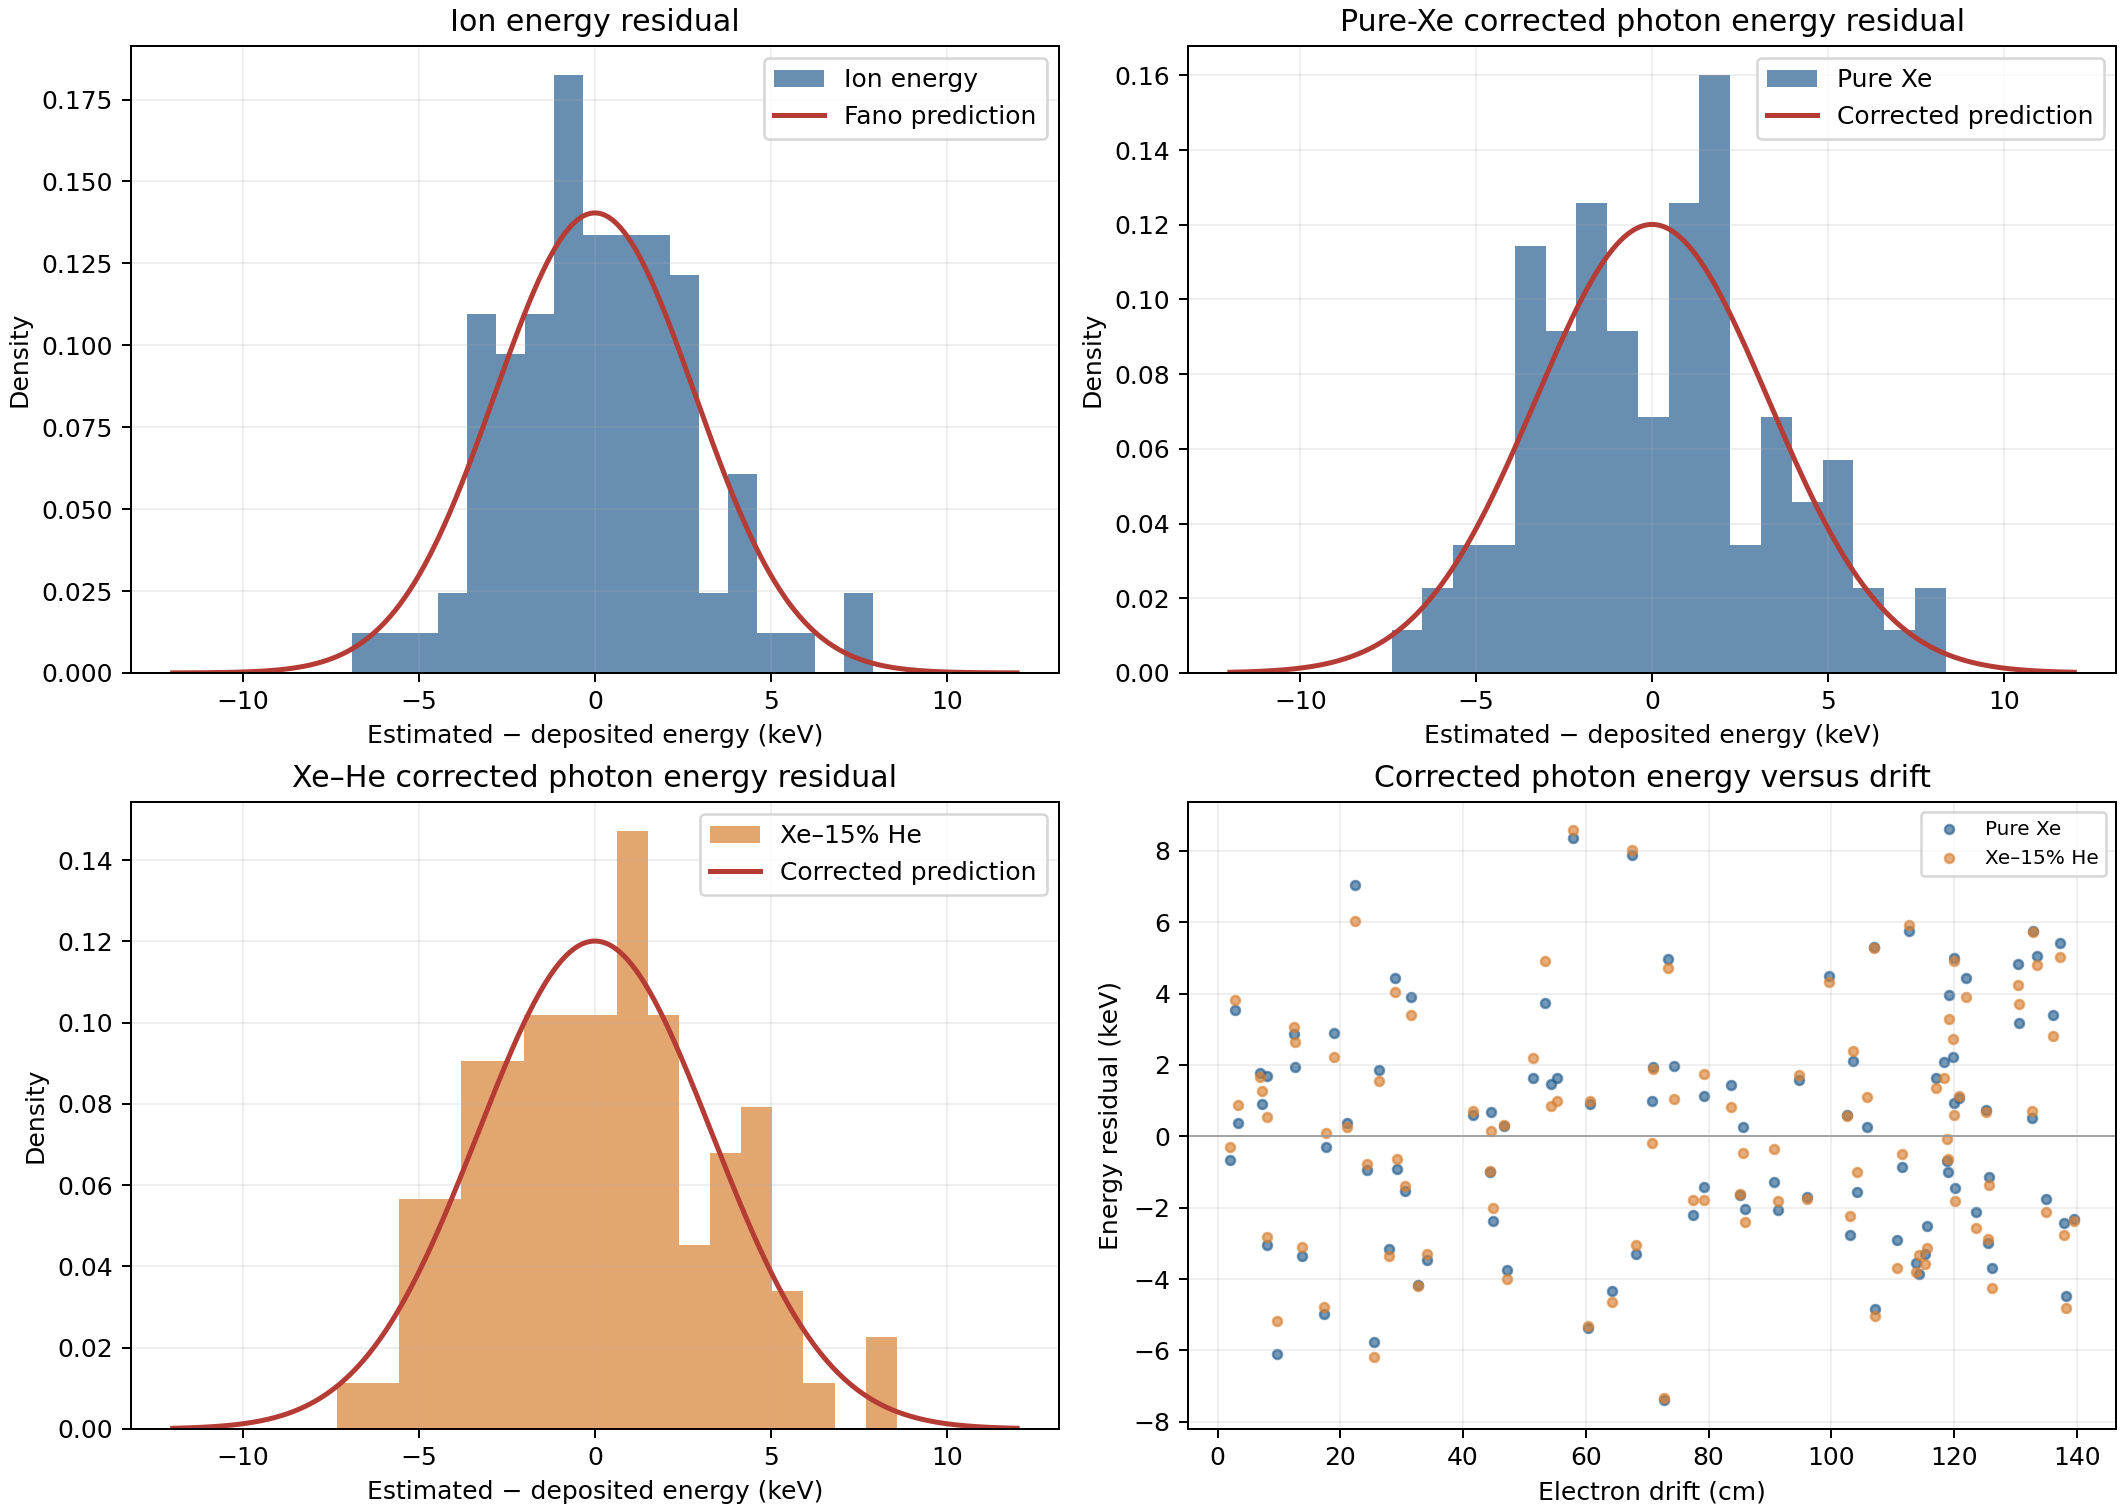
\includegraphics[width=0.98\linewidth]{total_fluctuations.png}\end{center}
\section*{Provenance}
Numerical HDF5 reduction: \texttt{total\_fluctuations\_bb0nu\_100\_41b93bb23acbe2ac.h5}. The reduction stores the source summary digest, cards' derived values, event IDs, drift lengths, observed counts and predicted conditional variances. The $F$ and $J$ definitions follow Oliveira et al., JINST 6 (2011) P05007; the adopted $J=0.01$ at $E/P=3$ is an approximate user reading of Figure 6.
\end{document}
